\documentclass{standalone}
\usepackage{tikz}
\usepackage{xcolor}

\begin{document}
	
	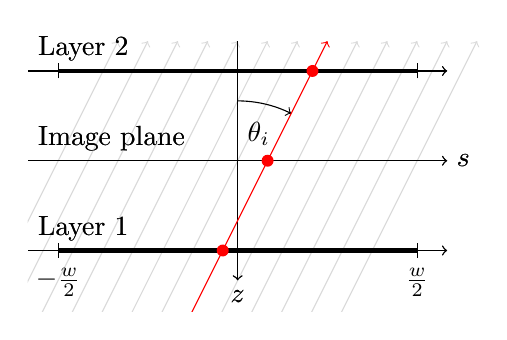
\begin{tikzpicture}[scale = 0.19,
						one end extended/.style = {shorten <= -#1},
		 				one end extended/.default = 1cm,
		 				]
	
		\colorlet{lightgray}{gray!30}
		
		% Sensor plane
		\draw[<-] (14, 0) -- (-14, 0);
		\node[right] at (14, 0) {$s$};
		
		% Top and bottom layer planes
		\draw[->] (-14, -6) -- (14, -6);
		\draw[->] (-14, 6) -- (14, 6);
		
		% z-axis
		\draw[->] (0, 8) -- (0, -8);
		\node[below] at (0, -8) {$z$};		
		
		% Labels for image plane and layers
		\node[above, anchor = south west] at (-14, 0) {Image plane};
		\node[above, anchor = south west] at (-14, 6) {Layer 2};
		\node[above, anchor = south west] at (-14, -6) {Layer 1};
		
		% Save current bounding box to clip light rays
		\coordinate (NE) at (current bounding box.north east);
		\coordinate (SW) at (current bounding box.south west);
		\clip (SW) rectangle (NE);
		
		\begin{scope}
%			\coordinate (R) at (-14, 14);
%			\clip (-14, 0 |- SW) rectangle (14, 0 |- NE);
		
			% Rays and intersections
			\draw[->, one end extended = 10cm, lightgray] (8, -8) -- (16, 8);
			\draw[->, one end extended = 10cm, lightgray] (6, -8) -- (14, 8);
			\draw[->, one end extended = 10cm, lightgray] (4, -8) -- (12, 8);
			\draw[->, one end extended = 10cm, lightgray] (2, -8) -- (10, 8);
			\draw[->, one end extended = 10cm, lightgray] (0, -8) -- (8, 8);
			
			\draw[->, one end extended = 10cm, lightgray] (-4, -8) -- (4, 8);
			\draw[->, one end extended = 10cm, lightgray] (-6, -8) -- (2, 8);
			\draw[->, one end extended = 10cm, lightgray] (-8, -8) -- (0, 8);
			\draw[->, one end extended = 10cm, lightgray] (-10, -8) -- (-2, 8);
			\draw[->, one end extended = 10cm, lightgray] (-12, -8) -- (-4, 8);
			\draw[->, one end extended = 10cm, lightgray] (-14, -8) -- (-6, 8);
			\draw[->, one end extended = 10cm, lightgray] (-14, -4) -- (-8, 8);
		\end{scope}
		
		\draw[ultra thick] (-12, -6) -- (12, -6);
		\draw[ultra thick] (-12, 6) -- (12, 6);
		
		% Draw lines of coordinate system again on top of rays
		\draw[<-] (14, 0) -- (-14, 0);
		\node[right] at (14, 0) {$s$};
		\draw[->] (-14, -6) -- (14, -6);
		\draw[->] (-14, 6) -- (14, 6);
		\draw[->] (0, 8) -- (0, -8);
		\node[below] at (0, -8) {$z$};
		
		% Angle and label
		\draw[->] (0, 4) arc (90 : atan(2) : 8);
		\node at (1.4, 1.8) {$\theta_i$};
		
		% Draw red ray on top of everything
		\draw[->, one end extended = 10cm, red] (-2, -8) -- (6, 8);	
		
		% Intersection markers
		\fill[red] (2, 0) circle[radius = 0.4];
		\fill[red] (5, 6) circle[radius = 0.4];
		\fill[red] (-1, -6) circle[radius = 0.4];	
		
		% Width markers
		\draw (-12, -0.5 + 6) -- (-12, 0.5 + 6);
		\draw (12, -0.5 + 6) -- (12, 0.5 + 6);
		\draw (-12, -0.5 - 6) -- (-12, 0.5 - 6);
		\draw (12, -0.5 - 6) -- (12, 0.5 - 6);
		\node[below] at (-12, -0.5 - 6) {$-\frac{w}{2}$};
		\node[below] at (12, -0.5 - 6) {$\frac{w}{2}$};
		
		% Draw again on top of gray lines
		\node[above, anchor = south west] at (-14, 0) {Image plane};
		\node[above, anchor = south west] at (-14, 6) {Layer 2};
		\node[above, anchor = south west] at (-14, -6) {Layer 1};
		
	\end{tikzpicture}
	
\end{document}